
%\chapter{Introduction}
\chapter{Introducere}
\label{cap:Introducere}


\section{Context}

In general, tentativele da expluatarea vulnerabilitatilor unei aplicatii vin sub forma de input catre aceasta, generate de catrea un atacator care intentioneaza sa intrerupa activitatea sau sa preia controlul aplicatiei. Un sitem de prevenire a intruziunilor (IPS) are rolul de a sta intre aplicatie si clientii acesteia, si de a prevenie expluatarea unor astfel de vulnerabilitati.

Prin folosirea unu reverse proxy pentru accesarea resurselor unui server de catre clineti, poate sa aduca numeroase beneficii procesului de administrare a serverului \cite{top_8}. Spre deosebire de un forward proxy care e un intermediar puntru un o serie de clienti prestabiliti, pentru a accesa orice server, un reverse proxy e un intermediar pentru o serie de servere prestabilite pentru a fi accesate de orice client. Unul dintre avantajele folosirii unui reverse proxy este centralizarea intregului trafic al serverului/serverelor intr-un singur punct de acces, aceasta fiind si principala caracteristica expluatata de acest proiect pentru filtrarea ip-urilor nedorite(in cazul nostru cele utilizate de reteaua Tor) si verificarea URI-urilor pentru posibile atacuri de SQL injection.

\begin{figure}[h]
	\centering
	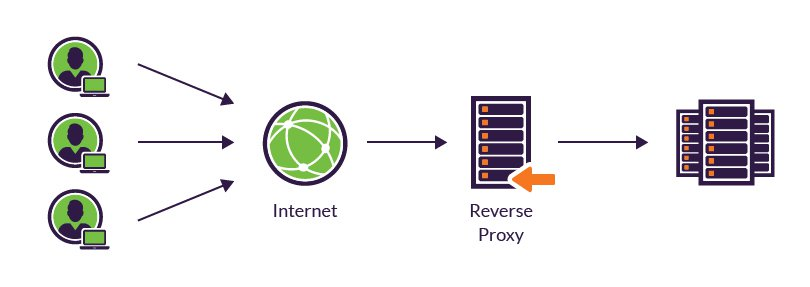
\includegraphics[width=0.5\textwidth]{reverse-proxy-02-1.jpg}
	\caption{Incapsula diagrama reverse proxy}
	\label{fig:reverse-proxy}
\end{figure}

Figura ~\ref{fig:reverse-proxy} ilustreaza modul de functionare al unui reverse proxy in relatie cu serverele aferente si posibili clienti. \\


Conform topului alcatuit de fundatia OWASP cu cele mai mari 10 riscuri ale aplicatiilor in 2017 \cite{owasp}, SQL injection e considerat a fi cea mai mare vulnerabilitate a aplicatiilor web. Acest lucru se datoreaza fatului ca mare parte din aceste aplicatii se bazeaza pe procesearea continutului furnizat de catre utilizatori. Atacurile de tipul SQL injection costau in faptul ca datele furnizate de catre utilizator sunt introduse in interogari SQL, unde acestea sunt tratate ca si cod executabil \cite{classification_and_countermeasures}. Aplicatiile web vulnerabile la sqli injection pot permite unor utilizatori neautorizati sa faca interogari intr-o baza de date asupra unor date la care nu ar avea acces in mod normal. Folosind acest tip de comportament neautorizat, un astfel de utilizator poate sa obtina accesul la informatii sensibile ale clientilor, dar si a administratorilor aplicatiei, precum credentiale sau date personale. Aceasta vulnerabilitate poate sa duca la furt de identitate sau frauda. 

In cazul retelei Tor, aceasta le permite utilizatorilor sa navigheze pe internet anonim. Anonimitatea online este importanta insa in multe cazuri aplicatiile web trebuie sa stie cine se conecteaza la aceasta pentru a le putea determina intentiile. Numele de Tor vine de la "the onion router" care sugereaza modul de operare al retelei. Fiecare participant la retea devine un nod de transfer, iar traficul retelei traverseaza o serie de astfel noduri pana sa ajunga la nodul de iesire ce creaza conexiunea cu destinatia dorita. Pachetele sunt criptate in mai multe "straturi", fiecare nod decriptand un singur strat de unde poate afla doar destinatia nodului urmator. Cand pachetul ajunge la ultimul nod, acesta trimite continutul la destinatie fara sa dezvalui identitatea sursei. Aceasta anonimitate usearaza desfasurarea atacurilor online. Conform datelor din reteaua organizatiei CloudFlare 94\% din traficul provenit din reteaua Tor este alcatuit din request-uri automate de origine malitioasa \cite{tor_trouble}.


%\section{Motivation}
 \section{Motivație}
In piata actuala exista multe sitem de prevenire a intruziunilor ce ofera atat caracteristicile unui reverse proxy, cat si cele de securitate. Aceste caracteristici sunt oferite fie ca si produse individualea, fie ca si produse ce le incorporeaza pe ambele. Cu toate acestea, produsele de acest gen sunt in general scumpe, au o logica mascata de detectarea a posibilelor probleme de securitate si sunt greu de inteles si de configurat de catre utilizator dupa propiile nevoi.

Prin oferirea utilizatorilor posibilitatea de a intelege si modifica modul de functionare a unui astfel de sistem poate rezulta in sisteme mult mai eficiente si rapide, dedicate pentru preferintele si nevoile aplicatiei fiacarui utilizator in parte. Spre exemplu, un utilizator poate sa decida ca nu are nevoie de funcionalitaile de detectie impotriva atacurilor de tip SQL injection pentru o anumita aplicatie, intrucat aceasta nu prezinta vulnerabilitati din acest punct de vedere, nefolosind o arhitectura bazata pe baze de date. In cazul acesta prin eliminarea unui astfel de modul, se elimina si verificarile aferente asupra reques-urilor clientilor, imbutatatind astfel performantele sistemului.

\textit{\thesistitle} ofera un sistem configurabil dupa preferintele utilizatorilor. Utilizatorul poate configura detectia bazata pe analiza request-ului primit de la client, acesta poate sa aleaga  care module sa fie folosite pentru detectie, permitand si eventuala adaugare de noi module(cat timp acestea respecta anumite conditii de structura), meniurile din interfata utilizator fiind generate in mod dinamic in functie de modelele prezente. Utilizator poate, de asemenea sa configureze si lista ip-urilior blocate, permitandu-i-se sastearga din cele existente, respectiva sa aduge unele noi, dupa bunul plac.



%\section{Report's Structure}
 \section{Structura lucrării}
In aceasta sectiune se prezinta structura lucrarii pe capitole si o scurta descriere a continutului acestora:

Primul capitol ~\ref{cap:Introducere}, prezinta o scurta introducere despre proiect, contextul acestuia si motivatia pentru implementarea sistemului propus.

Capitolul~\ref{cap:obiective-specificatii} prezinta obiectivele lucrarii, specificatiile sitemului, motivand deciziile luate in implementarea sistemului, cerintele functionale si nonfunctionale necesare implementarii sistemului.

 Capitolul~\ref{cap:studiu-bibliografic} descrie alte abordari similare ale problemelor tratate de proiectul propus, prin evidentierea asemanarilor si diferentelor dintre acestea si se explica tehnologiile si metodele folosite de proiect.
 
In capitolul~\ref{cap:fund-teoretice} sunt evidentiate si explicate pe scurt aspectele teoretice pe care se bazeaza proiectul.

Capitolul~\ref{cap:analiza-si-proiectare} descrie design-ul proiectului si cuprinde: cerintele sistemului, specificatiile cazurilor de utilizare, arhitectura sistemului, comportamentul sistemului, datele utilizate de sistem, dependintele sistemului si algoritmi esentiali si metodele folosite. Descrierea acestora se realizeaza prin asocierea cu diagramelor aferente.
